\begin{figure}[h]
    \centering
    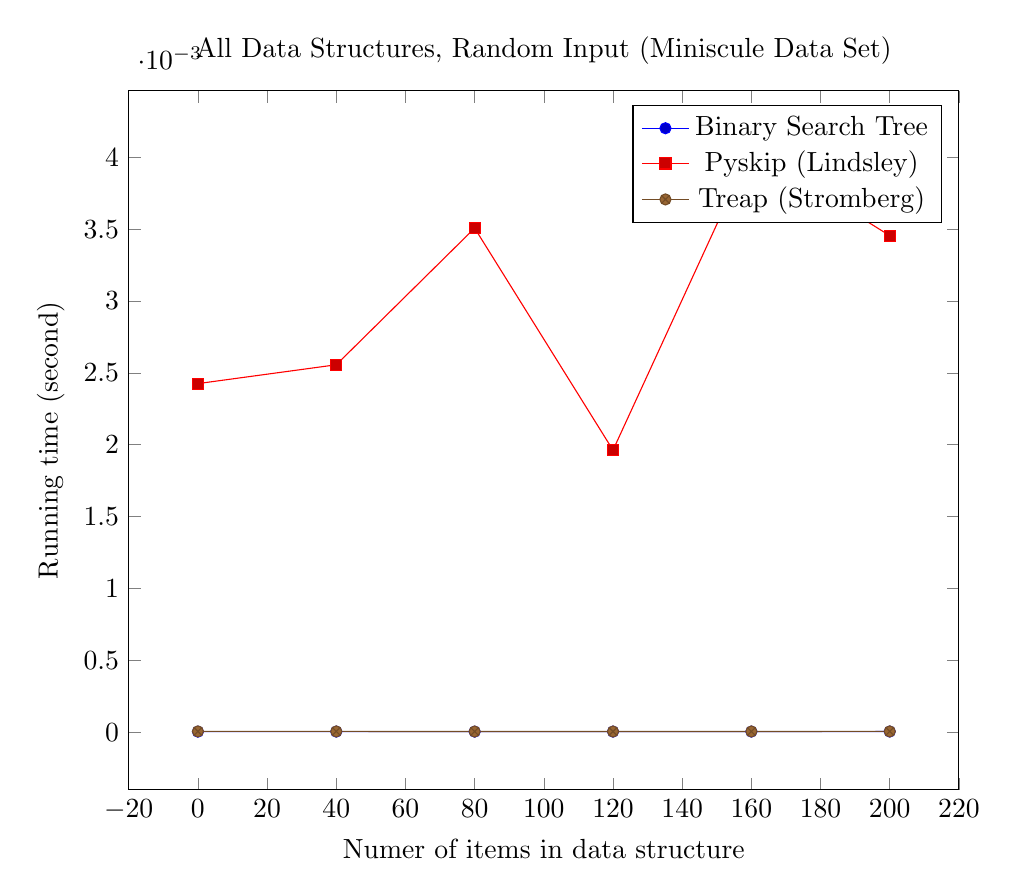
\begin{tikzpicture}
        \begin{axis}[
            xlabel={Numer of items in data structure},
            ylabel={Running time (second)},
            title={All Data Structures, Random Input (Miniscule Data Set)},
            width=\textwidth
        ]
		\addplot coordinates {
			(0, 3.7044566420396665e-06)
			(40, 4.035749512476538e-06)
			(80, 3.824926776752058e-06)
			(120, 4.0959845798216324e-06)
			(160, 4.12610211349973e-06)
			(200, 4.427277450247402e-06)
		};
		\addplot coordinates {
			(0, 0.0024251842816591764)
			(40, 0.0025561955531461455)
			(80, 0.003506855503602813)
			(120, 0.0019620970838698073)
			(160, 0.004056018612635803)
			(200, 0.0034545112300753632)
		};
		\addplot coordinates {
			(0, 5.481391128880908e-06)
			(40, 5.300685926812321e-06)
			(80, 4.607982652293785e-06)
			(120, 4.668217719649981e-06)
			(160, 4.939275522719555e-06)
			(200, 5.330803460501521e-06)
		};
        \legend{Binary Search Tree, Pyskip (Lindsley), Treap (Stromberg)}
        \end{axis}
    \end{tikzpicture}
    \caption{Average of 10 operations, benchmarked every 40, starting at 0.}
\end{figure}